\section{Structure}\label{sc:structure}
% Intro intro
Based on the analysis in the former sections, the structure of the classes in the problem domain has been visualised in a class diagram \autoref{fig:FirstPDClassDiagram}. 

\begin{figure}[H]
    \centering
    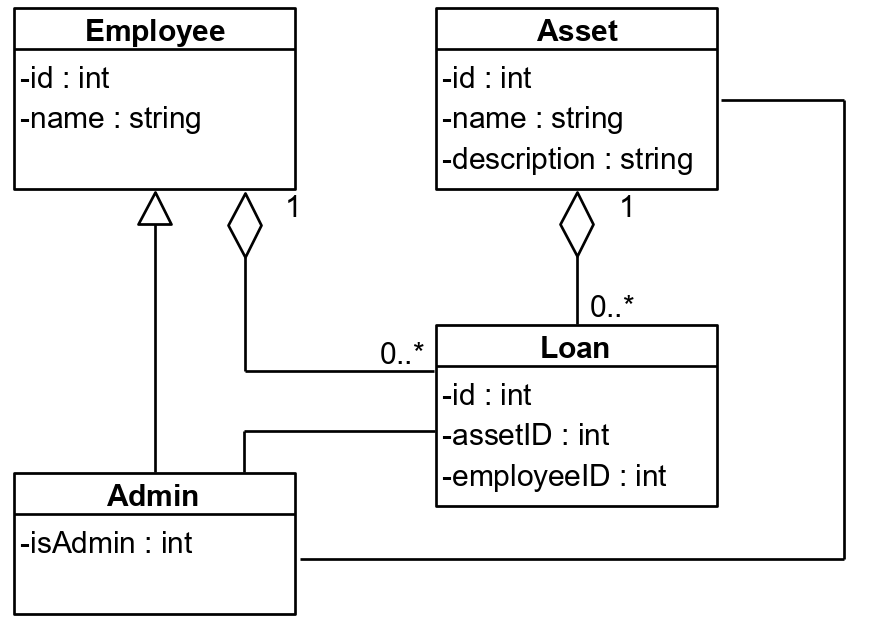
\includegraphics[width=0.8\textwidth]{figures/PDDiagramV5.png}
    \caption{Class diagram of the immediate classes in the problem domain.}
    \label{fig:FirstPDClassDiagram}
\end{figure}

As described in \autoref{sc:classes} there are 4 different classes. These classes are: Employee, Admin, Asset, and Loan. The relations between these has been described and justified below.
\par

The \textit{Employee} class is a super class, as it does not aggregate or generalize from any other classes. 
\par

The \textit{Asset} class is a super class as it does not aggregate or generalize from any other classes. The \textit{Asset} associates with the \textit{Admin} class as the \textit{Asset} stores which \textit{Admin} modified or created the \textit{Asset}.
\par

The \textit{Admin} class is a generalization from the \textit{Employee} class, as the \textit{Admin} class contains the same information as the \textit{Employee} class, but contains a boolean which gives a user with this class access to more functions in the system. The \textit{Admin} class also contains associations to assets and loans, as the admin users can create and modify these classes.
\par

The \textit{Loan} class is created to handle the relation in between the \textit{Asset} and \textit{Employee} class. The \textit{Loan} class aggregates from the \textit{Employee} class and the \textit{Asset} class, as this information is stored on the \textit{Loan} class upon creation.
\par

